% Forces one dimension
\section{Heildarkraftur}
Við getum skilgreint krafta til að vera $\uforce = \umass \uaccelea$, en
þegar við leggjum saman alla mismunandi krafta þá myndast \emph{heildarkraftur}.
Þá er allt talið saman, togkraftar, núningskraftar, þyngdarkraftar, o.s.f., til
að mynda kraft sem lýsir endanlegri hreyfingu hluta í lokuðu kerfi.
Heildarkrafturinn er gefinn sem summa allra krafta fyrir \emph{einn} hlut:
\begin{equation}
	\uforce_\text{heild} = \sum \text{allir kraftar} = \umass \uaccelea
\end{equation}
til að byrja með virkar þetta sem mjög óáhugaverð jafna en mun verða
talsvert hagnýtin með tímanum og sýnir styrk lögmála Newtons\footnote{
Táknið $\sum$ þýðir samanlagning, notast til að tákna
samanlagningu á stærðum (eða kröftum hér) }. 
\begin{center}
	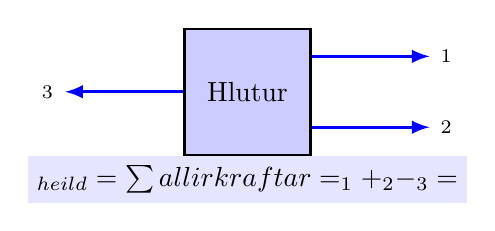
\begin{tikzpicture}[
		scale=1.5, 
		place/.style={rectangle,draw=black,fill=blue!20,thick,
		inner sep=0pt,minimum size=16mm},
		force/.style={>=latex,draw=blue,fill=blue, very thick, ->}
		]
		\node[place] (m) at (0,0) {Hlutur};
		\draw[force] (m.east) ++(0, 3mm)  -- ++(1,0) node[right] {$\uforce_1$};
		\draw[force] (m.east) ++(0, -3mm)  -- ++(1,0) node[right] {$\uforce_2$};
		\draw[force] (m.west) -- ++(-1,0) node[left] {$\uforce_3$};
		\node[below, fill=blue!10] (t) at (m.south)
			{
				$\uforce_\text{heild} 
					= \sum \text{allir kraftar} 
					=  \uforce_1 + \uforce_2 - \uforce_3
					= \umass \uaccelea
				$
			};
	\end{tikzpicture}
\end{center}
Aðalatriði í
beitingu heildarkraftsins er að velja sér hnitakerfi og byrja skilgreina
hvar mismunandi kraftar verka á ákveðin hlut. Þegar sagt er hnitakerfi
er átt við að velja hvað er jákvæð stefna í hreyfingu í láréttu og lóðréttu.
Til að reyna sýna hvernig á beita heildarkrafti er best að nýta sér
sýnidæmi.
\begin{formalexample}
Við höfum $\SI{10}{\kilo\gram}$ kassa sem liggur á borði, og er dreginn af 
$\SI{20}{\newton}$ krafti og það er $\SI{5}{\newton}$ kraftur sem verkar á móti hreyfingu 
kassans. Hver er heildarkrafturinn? Hver er hröðun kassans?
\\[4 ex]
Heildarkrafturinn er summa togkrafts $\SI{20}{\newton}$ og mótkraftur er 
$\SI{5}{\newton}$
sem gefur
\[
	\uforce_\text{heild} = \uforce_\text{tog} - \uforce_\text{mót}
		= \SI{20}{\newton} - \SI{5}{\newton} = \SI{15}{\newton}
\]
þar sem heildarkraftur er $\uforce_\text{heild} = \umass\uaccelea$, þá er hægt
að einangra hröðun hlutarins
\[
	\uforce_\text{heild} = \umass\uaccelea 
		\Leftrightarrow
		\uaccelea = \frac{\uforce_\text{heild}}{\umass}
			= \frac{ \SI{15}{\newton} }{ \SI{10}{\kilo\gram} }
			= \SI{1.5}{ \meter\per\second\squared }
\]
sem er þá hröðun kassans þegar allir kraftar eru taldir saman.
\end{formalexample}

\begin{formalexample}
Við höfum $\SI{1}{\kilo\gram}$ kúlu sem hangir í lausu lofti í bandi, og er toguð upp
með $\SI{20}{\newton}$ krafti, þyngdarkrafturinn verkar á móti
togkraftinum með stærðinni $\SI{9.8}{\newton}$. 
Hver er heildarkrafturinn? Hver er hröðun kúlunnar?
\\[4 ex]
Heildarkrafturinn er summa togkrafts $\SI{20}{\newton}$ og þyngdarkrafts sem 
er $\SI{9.8}{\newton}$
sem gefur
\[
	\uforce_\text{heild} = \uforce_\text{tog} - \uforce_\text{g}
		= \SI{20}{\newton} - \SI{9.8}{\newton} = \SI{10.2}{\newton}
\]
þar sem heildarkraftur er $\uforce_\text{heild} = \umass\uaccelea$, þá er hægt
að einangra hröðun hlutarins
\[
	\uforce_\text{heild} = \umass\uaccelea 
		\Leftrightarrow
		\uaccelea = \frac{\uforce_\text{heild}}{\umass}
			= \frac{
				\SI{10.2}{\newton}
				}{
				\SI{1}{\kilo\gram}
				}
			= \SI{10.2}{\meter\per\second\squared}
\]
sem er þá hröðun kúlunnar þegar allir kraftar eru taldir saman.
\end{formalexample}
aftur á móti eru nokkur önnur sértilfelli af þessu lögmáli. \emph{Þegar við tölum um
jafnan hraða getum við sagt að hraði hlutar helst óbreyttur}. Þetta gefur að
\[
	\uforce_\text{heild} = \umass \cdot \SI{0}{\meter\per\second\squared} 
		= \SI{0}{\newton}
\]
sem gildir bara fyrir hluti sem ferðast með \emph{óbreyttum} hraða. Sem dæmi er
\begin{formalexample}
Við höfum $\SI{1}{\kilo\gram}$ kúlu sem hangir í lausu lofti í bandi, og er toguð upp
með krafti og heldur kúlunni á jöfnum hraða, þyngdarkrafturinn verkar á móti
togkraftinum með stærðinni $\SI{9.8}{\newton}$. 
Hver er togkrafturinn? 
\\[4 ex]
Heildarkrafturinn er summa togkrafts og þyngdarkrafts sem er 
$\SI{9.8}{\newton}$, 
samanlagt verður heildarkrafturinn $\SI{0}{\newton}$ til að halda
kúlunni á jöfnum hraða. Sem gefur
\[
	\uforce_\text{heild} = \uforce_\text{tog} - \uforce_\text{g} = \SI{0}{\newton}
	\Leftrightarrow
	\uforce_\text{tog} - \SI{9.8}{\newton} = \SI{0}{\newton}
	\Leftrightarrow
	\uforce_\text{tog} = \SI{9.8}{\newton}
\]
þ.e.a.s. togkrafturinn er jafn stór og þyngdarkrafturinn ef við höldum kúlunni
á jöfnum hraða. Athugið að jafn hraði oft losar sig við fullt af vandamálum og
einfaldar talsvert kraftasamhengi.
\end{formalexample}

\section{Þyngdarkraftur}
Stærð þyngdarkraftsins er í samræmi við massa hlutars, þetta er langdregin leið
til að segja hlutur með meira massa veldur stærri þyngdarkrafti. Mátinn sem við
getum lagt fram stærð þyngdarkrafts sem er:
\begin{equation}
	\uforce_\text{\uacceleg} = \umass \uacceleg
\end{equation}
þar sem $\uacceleg = \SI{9.8}{\meter\per\second\squared}$. 
\begin{center}
	\begin{tikzpicture}[
		scale=1.5, 
		place/.style={rectangle,draw=black,fill=blue!20,thick,
		inner sep=0pt,minimum size=16mm},
		force/.style={>=latex,draw=blue,fill=blue, very thick, ->}
		]
		\node[place] (m) at (0,0) {Hlutur};
		\draw[fill = blue!40] (m.south) 
			++(-10mm, 0mm) 
			rectangle(10mm, -5mm)
			; 
		\draw[force] (m.center) -- ++(0,-8mm) node[below] {$\uforce_\uacceleg$};
	\end{tikzpicture}
\end{center}
Þá er einungis að ræða um hröðun sem hlutur
upplifir vegna þyngdarsviðs jarðar (og á yfirborði jarðar samtímis).
Þyngdarhröðun er breytileg milli pláneta, þess vegna er talað um \emph{þyngd} 
hlutars í Newtons og \emph{massa} hlutar í kílógrömmum. Massi hlutar er óháður 
þyngdarsviðinu, en þyngdin er háð styrk þyngdarsviðsins.
\begin{formalexample}
Við höfum $\SI{5}{\kg}$ kúlu sem hangir í lausu lofti í bandi, og er toguð upp
með krafti og heldur kúlunni á jöfnum hraða. Hver er togkrafturinn? 
\\[4 ex]
Við getum nýtt fyrri dæmi þar sem kúlan er á \emph{jöfnum} hraða, þá er hægt að segja
\[
	\uforce_\text{tog} = \uforce_\text{g}
\]
og þar sem við höfum nýlega skilgreint stærð þyngdarkrafts, þá er
\[
	\uforce_\text{tog} = \uforce_\text{g} = \umass \uacceleg 
		= \SI{5}{\kg} \times \SI{9.8}{\meter\per\second\squared}
		= \SI{49}{\newton}
\]
\end{formalexample}

\section{Þverkraftur}
Þegar kraftur verkar á yfirborð hluta, þá myndast gagnstæður kraftur sem er 
kallaður þverkraftur. Til samanburðar, ef bók liggur á borði, þá er það
þverkrafturinn sem sér til þess að bókin dettur ekki í gegnum borðið. Í raun
er þverkraftur form af þriðja lögmáli Newtons.
\begin{formalexample}
Við höfum kyrrstæðan kassa sem liggur á borði (á láréttu plani), kassinn 
er $\SI{10}{\kg}$.
Hver er stærð þverkraftsins?
\\[4 ex]
Þar sem kassinn er kyrrstæður, þá getum við sagt að heildarkrafturinn meðfram
hinu lóðrétta sé núll. S.s. kassinn eykur hvorki hraðan sinn upp né niður. Sem
gefur að
\[
	\uforce_\text{heild} = \uforce_\text{þver} - \uforce_\text{g} 
		= \SI{0}{\newton}
	\Leftrightarrow \uforce_\text{þver} = \uforce_\text{g}
\]
og þar sem við þekkjum massa kassans þá er hægt að setja
\[
	\uforce_\text{þver} = \uforce_\text{g} 
		= \umass \uacceleg
		= \SI{10}{\kg} \times \SI{9.8}{\meter\per\second\squared}
		= \SI{98}{\newton}
\]
sem er þá þverkrafturinn sem kassinn upplifir vegna þyngdarkraftsins.
\end{formalexample}

\section{Núningskraftur}
Þegar hlutir ferðast yfir yfirborð, þá myndast kraftur verkar á
móti hreyfingu hlutarins. Sá kraftur kallast \emph{núningskraftur} og er í
hlutfalli við stærð þverkraftsins. Til að lýsa hversu stór prósenta af
þverkraftinum nýtist til að verða núningskraftur höfum við núningsstuðullinn 
$\mu$. Sem er notaður í samhengið
\begin{equation}
	\uforce_\text{nún} = \mu \uforce_\text{þver}
\end{equation}
núningskrafturinn sjálfur er afleiða þess að draga hlut eftir yfirborði. Ef
hluturinn er ekki á hreyfingu (eða reynir ekki að hreyfa sig) þá myndast ekki
núningskraftur. Ber að athuga núningsstuðullinn er \emph{einingarlaus} stærð, 
sem liggur á milli núll og einn.
\begin{formalexample}
Kassi er togaður áfram með jöfnum hraða á borði, núningsstuðull á milli borðs
og kassa er $0,4$, massi kassans er $\SI{5}{\kg}$.
Hver er stærð togkraftsins?
\\[4 ex]
Þar sem kassinn er á jöfnum hraða er $\uforce_\text{nún} = \uforce_\text{tog}$,
og þar sem kassinn liggur í láréttu plani þá er $\uforce_\text{þver} 
= \uforce_\text{nún}$. Sem gefur að
\[
	\uforce_\text{tog} = \uforce_\text{nún} 
		= \mu \uforce_\text{þver}
		= \mu \uforce_\text{g}
		= \mu \umass \uacceleg
		= 0,4 \times \SI{5}{\kg} \times \SI{9.8}{\meter\per\second\squared}
		= \SI{19.6}{\newton}
\]
sem gildir einungis í lárréttu plani með kassa á jöfnum hraða.
\end{formalexample}

\section{Gagnkraftur}
Sem stærð kemur hún sjálfkrafa þegar kraftur verkar á hlut, gagnkraftur sér til þess
að þegar kraftur verkar á hlut muntu finna fyrir því að kraftur sé beittur. Sem dæmi
er hægt að ímynda sér að ýta kassa úr kyrrstöðu, ef þú verkar á kassann með krafti þá ferðast
hluturinn áfram en ef það væri \emph{enginn} kraftur sem verkaði á móti myndi sá sem
ýtir kassanum ekki finna fyrir því. Sem er ókunnugt frá daglegri reynslu, ef ýtt er á
kassa þá finnst kraftur á móti, sem er kunnugt frá daglegri reynslu.

\begin{formalexample}
\begin{wrapfigure}{r}{0.25\textwidth}
	\vspace{-20pt}
	\begin{center}
	\begin{tikzpicture}[
		force/.style={>=latex,draw=blue,fill=blue, very thick},
		m/.style={circle,draw=black,fill=gray,minimum size=0.3cm,thin},
		scale=1
	]
		\node[m] (m) at (0,0) {};
		\draw[very thick, draw=black] (m.north) -- +(0,1.5);
		\draw[force, ->] (m.north) ++(0,1.5) -- +(0,0.50) node[above] {$\uforce_\text{tog}$};
		\draw[force, ->] (m.center) -- +(0,{-0.50}) node[below] {$\uforce_\uacceleg$};
		\draw[force, draw=red, fill=red, ->]
			(m.north) ++(0,1.45) -- +(0,{-0.50}) node[left] {$-\uforce_\text{taug}$};
		\draw[force, draw=red, fill=red, ->]
			(m.north) -- +(0,{0.50}) node[right] {$\uforce_\text{taug}$};
	\end{tikzpicture}
	\end{center}
	\vspace{-10pt}
\end{wrapfigure}
Kúla hangir í bandi, enda bandsins er haldið fast. Kúlan hefur massann 
$\SI{5}{\kg}$.
Sýndu stefnu og stærð allra krafta og gagnkrafta.
\\[4 ex]
Þar sem endinn á bandinu er haldið fast, þá er heildarkrafturinn núll, ef við skoðum
bara endann á bandinu þá eru kraftarnir verka á enda bandsins
\[
	\uforce_\text{heild,endi} = \uforce_\text{tog} - \uforce_\text{taug} 
	= \SI{0}{\newton} 
\]
og þar sem kúlan hengur í hinum endanum er
\[
	\uforce_\text{heild,kúla} = \uforce_\text{taug} - \uforce_\text{g} 
	= \SI{0}{\newton}
\]
núna er hægt að búa til heildar-kraftsmynd þar sem allir kraftarnir eru lagðir saman.
Ef við leggjum alla kraftana saman á samtímis
\begin{align*}
	\uforce_\text{heild} &= \uforce_\text{tog} 
		+ \uforce_\text{taug} 
		- \uforce_\text{taug} - \uforce_\text{g}
	= 0 \\
	\uforce_\text{heild} &= \uforce_\text{tog} 
		- \uforce_\text{g}
	= 0 \\
	\uforce_\text{tog} &= \uforce_\text{g}
\end{align*}
sem gefur að togkrafturinn er
\[
	\uforce_\text{tog} = \uforce_\text{g} = \umass \uacceleg 
		= \SI{5}{\kg} \times \SI{9.8}{\meter\per\second\squared}
		= \SI{49}{\newton}
\]
\end{formalexample}

\subsection{Heildarkraftur á stór kerfi}
Hingað til hefur verið unnið með ekki meira en einn hlut í einu, þá eru allir
kraftar sem verka á einn hlut teknir og lagðir saman til að mynda þann kraft sem
kemur ef allt er talið saman. En það er sjaldan sem það er svo einfalt
í raunveruleikanum, þá munu fleiri en einn hlutur oft taka þátt í því að mynda
heildarkraft. Nánar tiltekið þá er mikilvægt að bæta við massanum á hverjum hlut
sem er í kerfinu. Sem gefur
\begin{equation}
	\uforce_\text{heild} = \sum \text{allir kraftar} = \sum \umass \uaccelea
\end{equation}
sem þýðir að allir massar þurfa eru lagðir saman til að lýsa hreyfingu og
kröftum kerfisins, og samtímis táknar summu alla krafta. Nokkur dæmi eru heppileg til að
sýna hvernig slíkir eiginleikar lýsa sér.
\begin{formalexample}
\begin{wrapfigure}{r}{0.25\textwidth}
	\vspace{-20pt}
	\begin{center}
	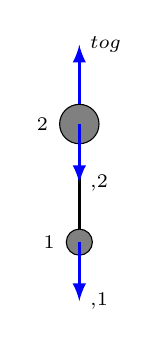
\begin{tikzpicture}[
		force/.style={>=latex,draw=blue,fill=blue, very thick},
		m1/.style={circle,draw=black,fill=gray,minimum size=0.3cm,thin},
		m2/.style={circle,draw=black,fill=gray,minimum size=0.5cm,thin},
		scale=1
	]
		\draw[very thick, draw=black] (0,0) -- +(0,1.5);
		\node[m1] (m1) at (0,0) {};
		\node[m2] (m2) at (0,1.5) {};
		\draw[] (m2.west) node[left] {$\umass_2$};
		\draw[] (m1.west) node[left] {$\umass_1$};
		\draw[force, ->] (m2.north) -- +(0,0.75) node[right] {$\uforce_\text{tog}$};
		\draw[force, ->] (m2.center) -- +(0,{-0.75}) node[right] {$\uforce_{\uacceleg,2}$};
		\draw[force, ->] (m1.center) -- +(0,{-0.75}) node[right] {$\uforce_{\uacceleg,1}$};
	\end{tikzpicture}
	\end{center}
	\vspace{-10pt}
\end{wrapfigure}
Kúlur hanga í bandi, enda bandsins er haldið fast. Kúla 1 hefur massann 
$\SI{2}{\kg}$. Kúla 2 hefur massan $\SI{5}{\kg}$. Sýndu stefnu og stærð 
allra krafta og gagnkrafta.
\\[4 ex]
Þar sem endinn á bandinu er haldið fast, þá er heildarkrafturinn núll, kraftarnir
sem verka á sitt hvora kúluna eru
\[
	\uforce_\text{heild,1} = \uforce_\text{taug} - \uforce_{\uacceleg,1} 
	= \SI{0}{\newton}
\]
og þar sem kúlan hengur í hinum endanum er
\[
	\uforce_\text{heild,2} = \uforce_\text{tog} 
		- \uforce_{\uacceleg,2} - \uforce_\text{taug} 
	= \SI{0}{\newton}
\]
núna er hægt að búa til heildar-kraftsmynd þar sem allir kraftarnir eru lagðir saman.
Ef við leggjum alla kraftana saman á samtímis
\begin{align*}
	\uforce_\text{heild} &= \uforce_\text{taug} - \uforce_{\uacceleg,1}
		+ \uforce_\text{tog} - \uforce_{\uacceleg,2} - \uforce_\text{taug}
		= \SI{0}{\newton} \\
	\uforce_\text{heild} &= \uforce_\text{tog} - \uforce_{\uacceleg,1}
		- \uforce_{\uacceleg,2} 
		= \SI{0}{\newton} \\
	\uforce_\text{heild} &= \uforce_\text{tog} - \umass_1 \uacceleg
		- \umass_2 \uacceleg
		= \SI{0}{\newton} \\
	\uforce_\text{heild} &= \uforce_\text{tog} - \SI{19.6}{\newton}
		- \SI{49}{\newton}
		= \SI{0}{\newton} \\
	\uforce_\text{tog} &= \SI{19.6}{\newton}
		+ \SI{49}{\newton}
		\\
	 &= \SI{68.6}{\newton}
\end{align*}
\end{formalexample}
Hins vegar er hægt að taka sömu aðstæður og í fyrra sýnidæmi og skoða hver
hröðunin verður ef togað er upp með krafti.
\begin{formalexample}
\begin{wrapfigure}{r}{0.25\textwidth}
	\vspace{-20pt}
	\begin{center}
	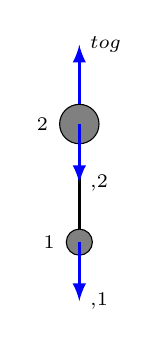
\begin{tikzpicture}[
		force/.style={>=latex,draw=blue,fill=blue, very thick},
		m1/.style={circle,draw=black,fill=gray,minimum size=0.3cm,thin},
		m2/.style={circle,draw=black,fill=gray,minimum size=0.5cm,thin},
		scale=1
	]
		\draw[very thick, draw=black] (0,0) -- +(0,1.5);
		\node[m1] (m1) at (0,0) {};
		\node[m2] (m2) at (0,1.5) {};
		\draw[] (m2.west) node[left] {$\umass_2$};
		\draw[] (m1.west) node[left] {$\umass_1$};
		\draw[force, ->] (m2.north) -- +(0,0.75) node[right] {$\uforce_\text{tog}$};
		\draw[force, ->] (m2.center) -- +(0,{-0.75}) node[right] {$\uforce_{\uacceleg,2}$};
		\draw[force, ->] (m1.center) -- +(0,{-0.75}) node[right] {$\uforce_{\uacceleg,1}$};
	\end{tikzpicture}
	\end{center}
	\vspace{-10pt}
\end{wrapfigure}
Kúlur hanga í bandi, enda bandsins er haldið fast. Kúla 1 hefur massann $\SI{2}{\kg}$.
Kúla 2 hefur massann $\SI{5}{\kg}$. Togað er í efri kúluna með 
$\SI{75}{\newton}$ krafti.
Sýndu stefnu og stærð allra krafta og gagnkrafta.
\\[4 ex]
Þar sem endinn á bandinu er haldið fast, þá er heildarkrafturinn núll, kraftarnir
sem verka á sitt hvora kúluna eru
\[
	\uforce_\text{heild,1} = \uforce_\text{taug} - \uforce_{\uacceleg,1} = \umass_\text{1} \uaccelea
\]
og þar sem kúlan hangir í hinum endanum er
\[
	\uforce_\text{heild,2} = \uforce_\text{tog} 
		- \uforce_{\uacceleg,2} - \uforce_\text{taug} = \umass_\text{2} \uaccelea
\]
núna er hægt að búa til heildar-kraftsmynd þar sem allir kraftarnir eru lagðir saman.
Ef við leggjum alla kraftana saman 
\begin{align*}
	\uforce_\text{heild} &= \uforce_\text{taug} - \uforce_{\uacceleg,1}
		+ \uforce_\text{tog} - \uforce_{\uacceleg,2} - \uforce_\text{taug}
		= \SI{0}{\newton} \\
	\uforce_\text{heild} &= \uforce_\text{tog} - \uforce_{\uacceleg,1}
		- \uforce_{\uacceleg,2} 
		= \left( \umass_\text{1} + \umass_\text{2}\right)  \uaccelea \\
	\uforce_\text{heild} &= \uforce_\text{tog} - \umass_1 \uacceleg
		- \umass_2 \uacceleg
		= \left( \umass_\text{1} + \umass_\text{2}\right)  \uaccelea \\
	\uforce_\text{heild} &= \SI{75}{\newton} - \SI{19.6}{\newton}
		- \SI{49}{\newton}
		= \left( \SI{7}{\kg} \right) \times \uaccelea \\
	\uforce_\text{heild} &= \SI{6.4}{\newton} 
		= \left( \SI{7}{\kg} \right) \times \uaccelea \\
	\uaccelea &= \frac{ \SI{6.4}{\newton} }{ \SI{7}{\kg} }
		\\
		&= \SI{0.914}{\meter\per\second\squared}
\end{align*}
\end{formalexample}
